\pgfdeclareplotmark{cross} {
\pgfpathmoveto{\pgfpoint{-0.3\pgfplotmarksize}{\pgfplotmarksize}}
\pgfpathlineto{\pgfpoint{+0.3\pgfplotmarksize}{\pgfplotmarksize}}
\pgfpathlineto{\pgfpoint{+0.3\pgfplotmarksize}{0.3\pgfplotmarksize}}
\pgfpathlineto{\pgfpoint{+1\pgfplotmarksize}{0.3\pgfplotmarksize}}
\pgfpathlineto{\pgfpoint{+1\pgfplotmarksize}{-0.3\pgfplotmarksize}}
\pgfpathlineto{\pgfpoint{+0.3\pgfplotmarksize}{-0.3\pgfplotmarksize}}
\pgfpathlineto{\pgfpoint{+0.3\pgfplotmarksize}{-1.\pgfplotmarksize}}
\pgfpathlineto{\pgfpoint{-0.3\pgfplotmarksize}{-1.\pgfplotmarksize}}
\pgfpathlineto{\pgfpoint{-0.3\pgfplotmarksize}{-0.3\pgfplotmarksize}}
\pgfpathlineto{\pgfpoint{-1.\pgfplotmarksize}{-0.3\pgfplotmarksize}}
\pgfpathlineto{\pgfpoint{-1.\pgfplotmarksize}{0.3\pgfplotmarksize}}
\pgfpathlineto{\pgfpoint{-0.3\pgfplotmarksize}{0.3\pgfplotmarksize}}
\pgfpathclose
\pgfusepathqstroke
}
\pgfdeclareplotmark{cross*} {
\pgfpathmoveto{\pgfpoint{-0.3\pgfplotmarksize}{\pgfplotmarksize}}
\pgfpathlineto{\pgfpoint{+0.3\pgfplotmarksize}{\pgfplotmarksize}}
\pgfpathlineto{\pgfpoint{+0.3\pgfplotmarksize}{0.3\pgfplotmarksize}}
\pgfpathlineto{\pgfpoint{+1\pgfplotmarksize}{0.3\pgfplotmarksize}}
\pgfpathlineto{\pgfpoint{+1\pgfplotmarksize}{-0.3\pgfplotmarksize}}
\pgfpathlineto{\pgfpoint{+0.3\pgfplotmarksize}{-0.3\pgfplotmarksize}}
\pgfpathlineto{\pgfpoint{+0.3\pgfplotmarksize}{-1.\pgfplotmarksize}}
\pgfpathlineto{\pgfpoint{-0.3\pgfplotmarksize}{-1.\pgfplotmarksize}}
\pgfpathlineto{\pgfpoint{-0.3\pgfplotmarksize}{-0.3\pgfplotmarksize}}
\pgfpathlineto{\pgfpoint{-1.\pgfplotmarksize}{-0.3\pgfplotmarksize}}
\pgfpathlineto{\pgfpoint{-1.\pgfplotmarksize}{0.3\pgfplotmarksize}}
\pgfpathlineto{\pgfpoint{-0.3\pgfplotmarksize}{0.3\pgfplotmarksize}}
\pgfpathclose
\pgfusepathqfillstroke
}
\pgfdeclareplotmark{newstar} {
\pgfpathmoveto{\pgfqpoint{0pt}{\pgfplotmarksize}}
\pgfpathlineto{\pgfqpointpolar{44}{0.5\pgfplotmarksize}}
\pgfpathlineto{\pgfqpointpolar{18}{\pgfplotmarksize}}
\pgfpathlineto{\pgfqpointpolar{-20}{0.5\pgfplotmarksize}}
\pgfpathlineto{\pgfqpointpolar{-54}{\pgfplotmarksize}}
\pgfpathlineto{\pgfqpointpolar{-90}{0.5\pgfplotmarksize}}
\pgfpathlineto{\pgfqpointpolar{234}{\pgfplotmarksize}}
\pgfpathlineto{\pgfqpointpolar{198}{0.5\pgfplotmarksize}}
\pgfpathlineto{\pgfqpointpolar{162}{\pgfplotmarksize}}
\pgfpathlineto{\pgfqpointpolar{134}{0.5\pgfplotmarksize}}
\pgfpathclose
\pgfusepathqstroke
}
\pgfdeclareplotmark{newstar*} {
\pgfpathmoveto{\pgfqpoint{0pt}{\pgfplotmarksize}}
\pgfpathlineto{\pgfqpointpolar{44}{0.5\pgfplotmarksize}}
\pgfpathlineto{\pgfqpointpolar{18}{\pgfplotmarksize}}
\pgfpathlineto{\pgfqpointpolar{-20}{0.5\pgfplotmarksize}}
\pgfpathlineto{\pgfqpointpolar{-54}{\pgfplotmarksize}}
\pgfpathlineto{\pgfqpointpolar{-90}{0.5\pgfplotmarksize}}
\pgfpathlineto{\pgfqpointpolar{234}{\pgfplotmarksize}}
\pgfpathlineto{\pgfqpointpolar{198}{0.5\pgfplotmarksize}}
\pgfpathlineto{\pgfqpointpolar{162}{\pgfplotmarksize}}
\pgfpathlineto{\pgfqpointpolar{134}{0.5\pgfplotmarksize}}
\pgfpathclose
\pgfusepathqfillstroke
}
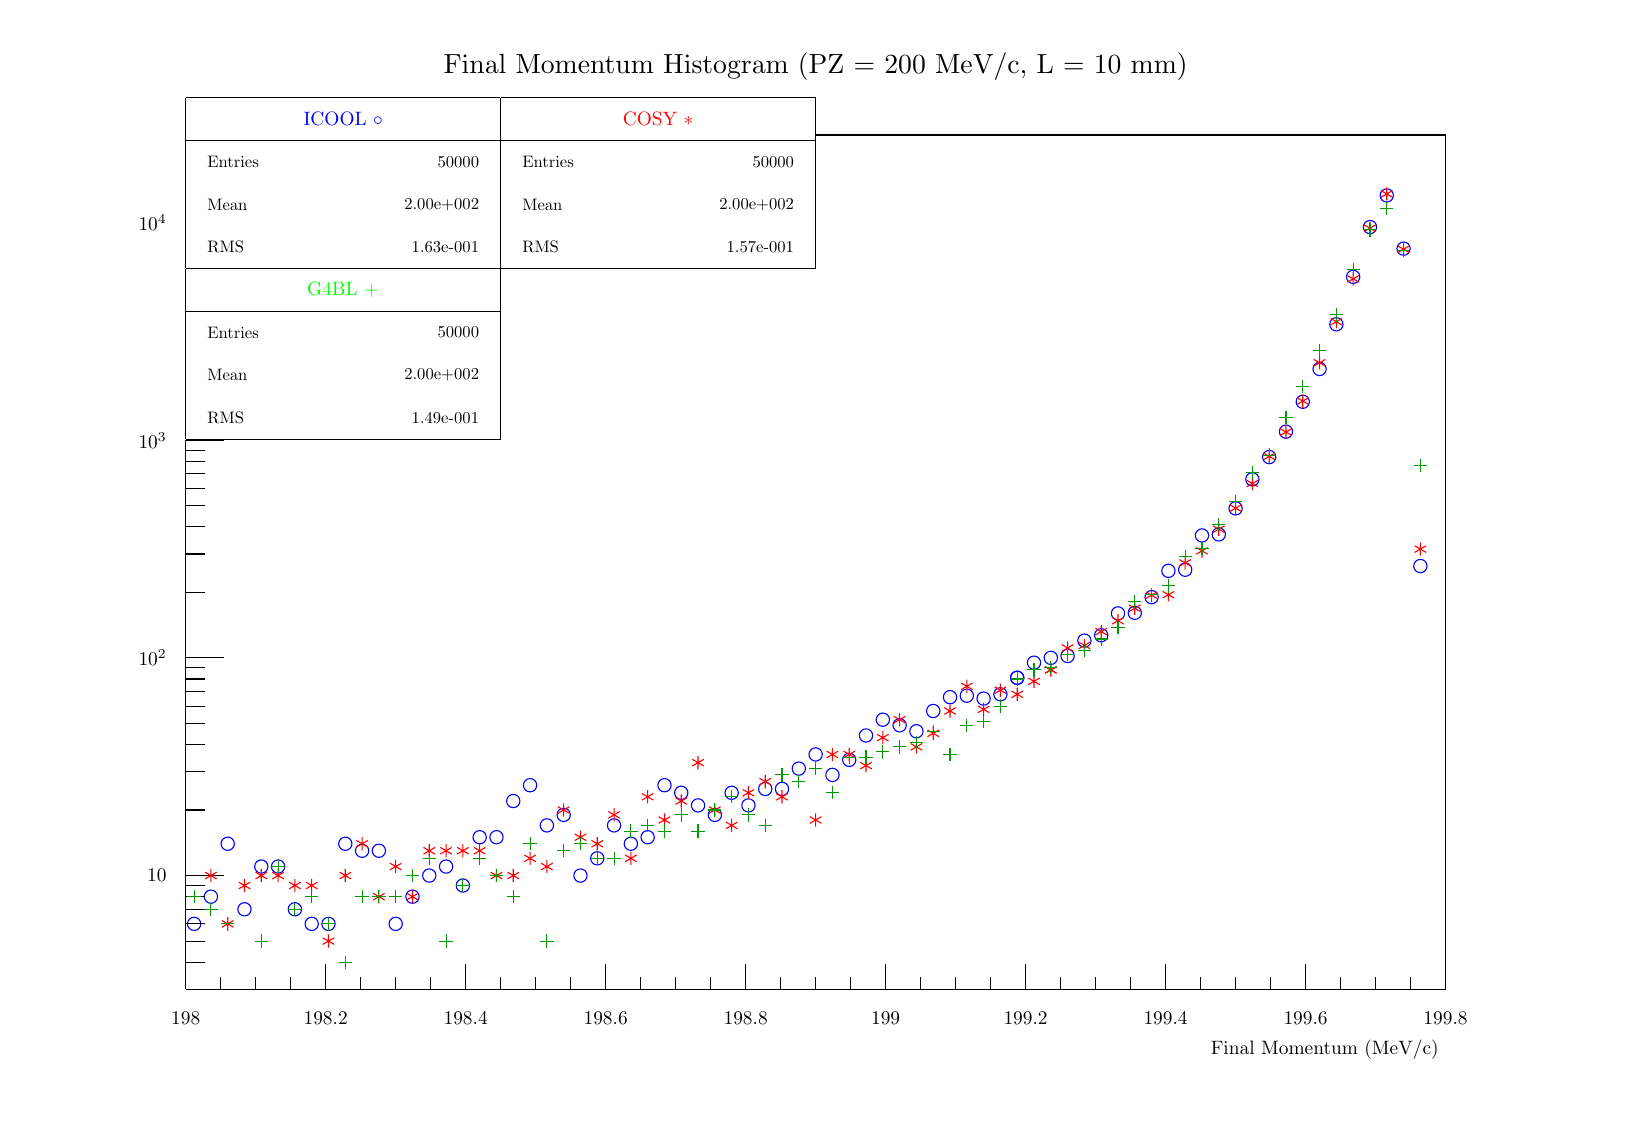
\begin{tikzpicture}
\definecolor{c}{rgb}{1,1,1};
\draw [color=c, fill=c] (0,0) rectangle (20,13.5632);
\draw [color=c, fill=c] (2,1.35632) rectangle (18,12.2069);
\definecolor{c}{rgb}{0,0,0};
\draw [c] (2,1.35632) -- (2,12.2069) -- (18,12.2069) -- (18,1.35632) -- (2,1.35632);
\definecolor{c}{rgb}{1,1,1};
\draw [color=c, fill=c] (2,1.35632) rectangle (18,12.2069);
\definecolor{c}{rgb}{0,0,0};
\draw [c] (2,1.35632) -- (2,12.2069) -- (18,12.2069) -- (18,1.35632) -- (2,1.35632);
\definecolor{c}{rgb}{0,0,1};
\foreach \P in
 {(2.10667,2.18864),(2.32,2.53408),(2.53333,3.20605),(2.74667,2.37374),(2.96,2.91647),(3.17333,2.91647),(3.38667,2.37374),(3.6,2.18864),(3.81333,2.18864),(4.02667,3.20605),(4.24,3.11707),(4.45333,3.11707),(4.66667,2.18864),(4.88,2.53408),(5.09333,2.8
0203),(5.30667,2.91647),(5.52,2.67551),(5.73333,3.2889),(5.94667,3.2889),(6.16,3.74879),(6.37333,3.94938),(6.58667,3.43919),(6.8,3.57275),(7.01333,2.80203),(7.22667,3.02095),(7.44,3.43919),(7.65333,3.20605),(7.86667,3.2889),(8.08,3.94938),(8.29333,3.
85327),(8.50667,3.69293),(8.72,3.57275),(8.93333,3.85327),(9.14667,3.69293),(9.36,3.90229),(9.57333,3.90229),(9.78667,4.16059),(10,4.34014),(10.2133,4.08051),(10.4267,4.27151),(10.64,4.5811),(10.8533,4.7817),(11.0667,4.71034),(11.28,4.63448),(11.4933
,4.89194),(11.7067,5.06798),(11.92,5.08603),(12.1333,5.04964),(12.3467,5.10382),(12.56,5.31389)}{\draw[mark options={color=c,fill=c},mark size=2.402402pt,mark=o] plot coordinates {\P};}
\foreach \P in
 {(12.56,5.31389),(12.7733,5.50533),(12.9867,5.56692),(13.2,5.5907),(13.4133,5.78585),(13.6267,5.85393),(13.84,6.13129),(14.0533,6.13877),(14.2667,6.33764),(14.48,6.67197),(14.6933,6.68624),(14.9067,7.1216),(15.12,7.13469),(15.3333,7.46539),(15.5467,
7.83469),(15.76,8.11672),(15.9733,8.43969),(16.1867,8.81949),(16.4,9.23579),(16.6133,9.80271),(16.8267,10.406),(17.04,11.0381),(17.2533,11.4395),(17.4667,10.7637),(17.68,6.73261)}{\draw[mark options={color=c,fill=c},mark size=2.402402pt,mark=o] plot
 coordinates {\P};}
\definecolor{c}{rgb}{1,1,1};
\draw [color=c, fill=c] (2,10.5115) rectangle (6,12.6816);
\definecolor{c}{rgb}{0,0,0};
\draw [c] (2,10.5115) -- (6,10.5115);
\draw [c] (6,10.5115) -- (6,12.6816);
\draw [c] (6,12.6816) -- (2,12.6816);
\draw [c] (2,12.6816) -- (2,10.5115);
\draw[color=blue](4,12.4103) node[scale=0.7, rotate=0]{ICOOL $\circ$};
\draw [c] (2,12.1391) -- (6,12.1391);
\draw [anchor= west] (2.2,11.8678) node[scale=0.6, rotate=0]{Entries };
\draw [anchor= east] (5.8,11.8678) node[scale=0.6, rotate=0]{ 50000};
\draw [anchor= west] (2.2,11.3253) node[scale=0.6, rotate=0]{Mean  };
\draw [anchor= east] (5.8,11.3253) node[scale=0.6, rotate=0]{ 2.00e+002};
\draw [anchor= west] (2.2,10.7828) node[scale=0.6, rotate=0]{RMS   };
\draw [anchor= east] (5.8,10.7828) node[scale=0.6, rotate=0]{ 1.63e-001};
\draw [c] (2,1.35632) -- (18,1.35632);
\draw [anchor= east] (18,0.596782) node[scale=0.7, rotate=0]{Final Momentum (MeV/c)};
\draw [c] (2,1.68184) -- (2,1.35632);
\draw [c] (2.44444,1.51908) -- (2.44444,1.35632);
\draw [c] (2.88889,1.51908) -- (2.88889,1.35632);
\draw [c] (3.33333,1.51908) -- (3.33333,1.35632);
\draw [c] (3.77778,1.68184) -- (3.77778,1.35632);
\draw [c] (4.22222,1.51908) -- (4.22222,1.35632);
\draw [c] (4.66667,1.51908) -- (4.66667,1.35632);
\draw [c] (5.11111,1.51908) -- (5.11111,1.35632);
\draw [c] (5.55556,1.68184) -- (5.55556,1.35632);
\draw [c] (6,1.51908) -- (6,1.35632);
\draw [c] (6.44444,1.51908) -- (6.44444,1.35632);
\draw [c] (6.88889,1.51908) -- (6.88889,1.35632);
\draw [c] (7.33333,1.68184) -- (7.33333,1.35632);
\draw [c] (7.77778,1.51908) -- (7.77778,1.35632);
\draw [c] (8.22222,1.51908) -- (8.22222,1.35632);
\draw [c] (8.66667,1.51908) -- (8.66667,1.35632);
\draw [c] (9.11111,1.68184) -- (9.11111,1.35632);
\draw [c] (9.55556,1.51908) -- (9.55556,1.35632);
\draw [c] (10,1.51908) -- (10,1.35632);
\draw [c] (10.4444,1.51908) -- (10.4444,1.35632);
\draw [c] (10.8889,1.68184) -- (10.8889,1.35632);
\draw [c] (11.3333,1.51908) -- (11.3333,1.35632);
\draw [c] (11.7778,1.51908) -- (11.7778,1.35632);
\draw [c] (12.2222,1.51908) -- (12.2222,1.35632);
\draw [c] (12.6667,1.68184) -- (12.6667,1.35632);
\draw [c] (13.1111,1.51908) -- (13.1111,1.35632);
\draw [c] (13.5556,1.51908) -- (13.5556,1.35632);
\draw [c] (14,1.51908) -- (14,1.35632);
\draw [c] (14.4444,1.68184) -- (14.4444,1.35632);
\draw [c] (14.8889,1.51908) -- (14.8889,1.35632);
\draw [c] (15.3333,1.51908) -- (15.3333,1.35632);
\draw [c] (15.7778,1.51908) -- (15.7778,1.35632);
\draw [c] (16.2222,1.68184) -- (16.2222,1.35632);
\draw [c] (16.6667,1.51908) -- (16.6667,1.35632);
\draw [c] (17.1111,1.51908) -- (17.1111,1.35632);
\draw [c] (17.5556,1.51908) -- (17.5556,1.35632);
\draw [c] (18,1.68184) -- (18,1.35632);
\draw [anchor=base] (2,0.908736) node[scale=0.7, rotate=0]{198};
\draw [anchor=base] (3.77778,0.908736) node[scale=0.7, rotate=0]{198.2};
\draw [anchor=base] (5.55556,0.908736) node[scale=0.7, rotate=0]{198.4};
\draw [anchor=base] (7.33333,0.908736) node[scale=0.7, rotate=0]{198.6};
\draw [anchor=base] (9.11111,0.908736) node[scale=0.7, rotate=0]{198.8};
\draw [anchor=base] (10.8889,0.908736) node[scale=0.7, rotate=0]{199};
\draw [anchor=base] (12.6667,0.908736) node[scale=0.7, rotate=0]{199.2};
\draw [anchor=base] (14.4444,0.908736) node[scale=0.7, rotate=0]{199.4};
\draw [anchor=base] (16.2222,0.908736) node[scale=0.7, rotate=0]{199.6};
\draw [anchor=base] (18,0.908736) node[scale=0.7, rotate=0]{199.8};
\draw [c] (2,1.35632) -- (2,12.2069);
\draw [c] (2.24,1.70176) -- (2,1.70176);
\draw [c] (2.24,1.96971) -- (2,1.96971);
\draw [c] (2.24,2.18864) -- (2,2.18864);
\draw [c] (2.24,2.37374) -- (2,2.37374);
\draw [c] (2.24,2.53408) -- (2,2.53408);
\draw [c] (2.24,2.67551) -- (2,2.67551);
\draw [c] (2.48,2.80202) -- (2,2.80202);
\draw [anchor= east] (1.844,2.80202) node[scale=0.7, rotate=0]{10};
\draw [c] (2.24,3.63434) -- (2,3.63434);
\draw [c] (2.24,4.12121) -- (2,4.12121);
\draw [c] (2.24,4.46666) -- (2,4.46666);
\draw [c] (2.24,4.7346) -- (2,4.7346);
\draw [c] (2.24,4.95353) -- (2,4.95353);
\draw [c] (2.24,5.13863) -- (2,5.13863);
\draw [c] (2.24,5.29897) -- (2,5.29897);
\draw [c] (2.24,5.4404) -- (2,5.4404);
\draw [c] (2.48,5.56692) -- (2,5.56692);
\draw [anchor= east] (1.844,5.56692) node[scale=0.7, rotate=0]{$10^{2}$};
\draw [c] (2.24,6.39923) -- (2,6.39923);
\draw [c] (2.24,6.88611) -- (2,6.88611);
\draw [c] (2.24,7.23155) -- (2,7.23155);
\draw [c] (2.24,7.4995) -- (2,7.4995);
\draw [c] (2.24,7.71842) -- (2,7.71842);
\draw [c] (2.24,7.90352) -- (2,7.90352);
\draw [c] (2.24,8.06387) -- (2,8.06387);
\draw [c] (2.24,8.2053) -- (2,8.2053);
\draw [c] (2.48,8.33181) -- (2,8.33181);
\draw [anchor= east] (1.844,8.33181) node[scale=0.7, rotate=0]{$10^{3}$};
\draw [c] (2.24,9.16413) -- (2,9.16413);
\draw [c] (2.24,9.651) -- (2,9.651);
\draw [c] (2.24,9.99644) -- (2,9.99644);
\draw [c] (2.24,10.2644) -- (2,10.2644);
\draw [c] (2.24,10.4833) -- (2,10.4833);
\draw [c] (2.24,10.6684) -- (2,10.6684);
\draw [c] (2.24,10.8288) -- (2,10.8288);
\draw [c] (2.24,10.9702) -- (2,10.9702);
\draw [c] (2.48,11.0967) -- (2,11.0967);
\draw [anchor= east] (1.844,11.0967) node[scale=0.7, rotate=0]{$10^{4}$};
\draw [c] (2.24,11.929) -- (2,11.929);
\definecolor{c}{rgb}{1,1,1};
\draw [color=c, fill=c] (2,10.5115) rectangle (6,12.6816);
\definecolor{c}{rgb}{0,0,0};
\draw [c] (2,10.5115) -- (6,10.5115);
\draw [c] (6,10.5115) -- (6,12.6816);
\draw [c] (6,12.6816) -- (2,12.6816);
\draw [c] (2,12.6816) -- (2,10.5115);
\draw[color=blue](4,12.4103) node[scale=0.7, rotate=0]{ICOOL $\circ$};
\draw [c] (2,12.1391) -- (6,12.1391);
\draw [anchor= west] (2.2,11.8678) node[scale=0.6, rotate=0]{Entries };
\draw [anchor= east] (5.8,11.8678) node[scale=0.6, rotate=0]{ 50000};
\draw [anchor= west] (2.2,11.3253) node[scale=0.6, rotate=0]{Mean  };
\draw [anchor= east] (5.8,11.3253) node[scale=0.6, rotate=0]{ 2.00e+002};
\draw [anchor= west] (2.2,10.7828) node[scale=0.6, rotate=0]{RMS   };
\draw [anchor= east] (5.8,10.7828) node[scale=0.6, rotate=0]{ 1.63e-001};
\draw (10,13.0816) node[scale=1, rotate=0]{Final Momentum Histogram (PZ = 200 MeV/c, L = 10 mm)};
\definecolor{c}{rgb}{1,0,0};
\foreach \P in
 {(2.32,2.80203),(2.53333,2.18864),(2.74667,2.67551),(2.96,2.80203),(3.17333,2.80203),(3.38667,2.67551),(3.6,2.67551),(3.81333,1.96971),(4.02667,2.80203),(4.24,3.20605),(4.45333,2.53408),(4.66667,2.91647),(4.88,2.53408),(5.09333,3.11707),(5.30667,3.1
1707),(5.52,3.11707),(5.73333,3.11707),(5.94667,2.80203),(6.16,2.80203),(6.37333,3.02095),(6.58667,2.91647),(6.8,3.63434),(7.01333,3.2889),(7.22667,3.20605),(7.44,3.57275),(7.65333,3.02095),(7.86667,3.80216),(8.08,3.50783),(8.29333,3.74879),(8.50667,
4.23566),(8.72,3.63434),(8.93333,3.43919),(9.14667,3.85327),(9.36,3.9947),(9.57333,3.80216),(10,3.50783),(10.2133,4.34014),(10.4267,4.34014),(10.64,4.19871),(10.8533,4.5535),(11.0667,4.7817),(11.28,4.43626),(11.4933,4.60809),(11.7067,4.89194),(11.92,
5.20536),(12.1333,4.91282),(12.3467,5.15566),(12.56,5.10382),(12.7733,5.26857),(12.9867,5.41342)}{\draw[mark options={color=c,fill=c},mark size=2.402402pt,mark=asterisk] plot coordinates {\P};}
\foreach \P in
 {(12.9867,5.41342),(13.2,5.69223),(13.4133,5.72426),(13.6267,5.90029),(13.84,6.03767),(14.0533,6.197),(14.2667,6.36266),(14.48,6.36883),(14.6933,6.77286),(14.9067,6.92548),(15.12,7.20115),(15.3333,7.46786),(15.5467,7.78082),(15.76,8.12531),(15.9733,
8.43419),(16.1867,8.82746),(16.4,9.3146),(16.6133,9.83576),(16.8267,10.3799),(17.04,11.0234),(17.2533,11.4588),(17.4667,10.7564),(17.68,6.9485)}{\draw[mark options={color=c,fill=c},mark size=2.402402pt,mark=asterisk] plot coordinates {\P};}
\definecolor{c}{rgb}{1,1,1};
\draw [color=c, fill=c] (6,10.5115) rectangle (10,12.6816);
\definecolor{c}{rgb}{0,0,0};
\draw [c] (6,10.5115) -- (10,10.5115);
\draw [c] (10,10.5115) -- (10,12.6816);
\draw [c] (10,12.6816) -- (6,12.6816);
\draw [c] (6,12.6816) -- (6,10.5115);
\draw [color=red](8,12.4103) node[scale=0.7, rotate=0]{COSY $*$};
\draw [c] (6,12.1391) -- (10,12.1391);
\draw [anchor= west] (6.2,11.8678) node[scale=0.6, rotate=0]{Entries };
\draw [anchor= east] (9.8,11.8678) node[scale=0.6, rotate=0]{ 50000};
\draw [anchor= west] (6.2,11.3253) node[scale=0.6, rotate=0]{Mean  };
\draw [anchor= east] (9.8,11.3253) node[scale=0.6, rotate=0]{ 2.00e+002};
\draw [anchor= west] (6.2,10.7828) node[scale=0.6, rotate=0]{RMS   };
\draw [anchor= east] (9.8,10.7828) node[scale=0.6, rotate=0]{ 1.57e-001};
\definecolor{c}{rgb}{1,1,1};
\draw [color=c, fill=c] (6,10.5115) rectangle (10,12.6816);
\definecolor{c}{rgb}{0,0,0};
\draw [c] (6,10.5115) -- (10,10.5115);
\draw [c] (10,10.5115) -- (10,12.6816);
\draw [c] (10,12.6816) -- (6,12.6816);
\draw [c] (6,12.6816) -- (6,10.5115);
\draw [color=red](8,12.4103) node[scale=0.7, rotate=0]{COSY $*$};
\draw [c] (6,12.1391) -- (10,12.1391);
\draw [anchor= west] (6.2,11.8678) node[scale=0.6, rotate=0]{Entries };
\draw [anchor= east] (9.8,11.8678) node[scale=0.6, rotate=0]{ 50000};
\draw [anchor= west] (6.2,11.3253) node[scale=0.6, rotate=0]{Mean  };
\draw [anchor= east] (9.8,11.3253) node[scale=0.6, rotate=0]{ 2.00e+002};
\draw [anchor= west] (6.2,10.7828) node[scale=0.6, rotate=0]{RMS   };
\draw [anchor= east] (9.8,10.7828) node[scale=0.6, rotate=0]{ 1.57e-001};
\definecolor{c}{rgb}{0,0.6,0};
\foreach \P in
 {(2.10667,2.53408),(2.32,2.37374),(2.53333,2.18864),(2.96,1.96971),(3.17333,2.91647),(3.38667,2.37374),(3.6,2.53408),(3.81333,2.18864),(4.02667,1.70176),(4.24,2.53408),(4.45333,2.53408),(4.66667,2.53408),(4.88,2.80203),(5.09333,3.02095),(5.30667,1.9
6971),(5.52,2.67551),(5.73333,3.02095),(5.94667,2.80203),(6.16,2.53408),(6.37333,3.20605),(6.58667,1.96971),(6.8,3.11707),(7.01333,3.20605),(7.22667,3.02095),(7.44,3.02095),(7.65333,3.3664),(7.86667,3.43919),(8.08,3.3664),(8.29333,3.57275),(8.50667,3
.3664),(8.72,3.63434),(8.93333,3.80216),(9.14667,3.57275),(9.36,3.43919),(9.57333,4.08051),(9.78667,3.9947),(10,4.16059),(10.2133,3.85327),(10.4267,4.30632),(10.64,4.30632),(10.8533,4.37304),(11.0667,4.43626),(11.28,4.49631),(11.4933,4.63448),(11.706
7,4.34014),(11.92,4.71034),(12.1333,4.75838),(12.3467,4.95353),(12.56,5.29897),(12.7733,5.41342)}{\draw[mark options={color=c,fill=c},mark size=2.402402pt,mark=+] plot coordinates {\P};}
\foreach \P in
 {(12.7733,5.41342),(12.9867,5.4404),(13.2,5.61401),(13.4133,5.65933),(13.6267,5.80569),(13.84,5.95367),(14.0533,6.27937),(14.2667,6.36883),(14.48,6.48048),(14.6933,6.85365),(14.9067,6.95229),(15.12,7.2612),(15.3333,7.5535),(15.5467,7.91717),(15.76,8
.1423),(15.9733,8.62354),(16.1867,9.01063),(16.4,9.46663),(16.6133,9.92214),(16.8267,10.4972),(17.04,11.0021),(17.2533,11.2773),(17.4667,10.74),(17.68,8.00543)}{\draw[mark options={color=c,fill=c},mark size=2.402402pt,mark=+] plot coordinates {\P};}
\definecolor{c}{rgb}{1,1,1};
\draw [color=c, fill=c] (2,8.34138) rectangle (6,10.5115);
\definecolor{c}{rgb}{0,0,0};
\draw [c] (2,8.34138) -- (6,8.34138);
\draw [c] (6,8.34138) -- (6,10.5115);
\draw [c] (6,10.5115) -- (2,10.5115);
\draw [c] (2,10.5115) -- (2,8.34138);
\draw [color=green](4,10.2402) node[scale=0.7, rotate=0]{G4BL $+$};
\draw [c] (2,9.96897) -- (6,9.96897);
\draw [anchor= west] (2.2,9.6977) node[scale=0.6, rotate=0]{Entries };
\draw [anchor= east] (5.8,9.6977) node[scale=0.6, rotate=0]{ 50000};
\draw [anchor= west] (2.2,9.15517) node[scale=0.6, rotate=0]{Mean  };
\draw [anchor= east] (5.8,9.15517) node[scale=0.6, rotate=0]{ 2.00e+002};
\draw [anchor= west] (2.2,8.61264) node[scale=0.6, rotate=0]{RMS   };
\draw [anchor= east] (5.8,8.61264) node[scale=0.6, rotate=0]{ 1.49e-001};
\definecolor{c}{rgb}{1,1,1};
\draw [color=c, fill=c] (2,8.34138) rectangle (6,10.5115);
\definecolor{c}{rgb}{0,0,0};
\draw [c] (2,8.34138) -- (6,8.34138);
\draw [c] (6,8.34138) -- (6,10.5115);
\draw [c] (6,10.5115) -- (2,10.5115);
\draw [c] (2,10.5115) -- (2,8.34138);
\draw [color=green](4,10.2402) node[scale=0.7, rotate=0]{G4BL $+$};
\draw [c] (2,9.96897) -- (6,9.96897);
\draw [anchor= west] (2.2,9.6977) node[scale=0.6, rotate=0]{Entries };
\draw [anchor= east] (5.8,9.6977) node[scale=0.6, rotate=0]{ 50000};
\draw [anchor= west] (2.2,9.15517) node[scale=0.6, rotate=0]{Mean  };
\draw [anchor= east] (5.8,9.15517) node[scale=0.6, rotate=0]{ 2.00e+002};
\draw [anchor= west] (2.2,8.61264) node[scale=0.6, rotate=0]{RMS   };
\draw [anchor= east] (5.8,8.61264) node[scale=0.6, rotate=0]{ 1.49e-001};
\end{tikzpicture}
